\section{構造}
\subsection{内骨格型グリッパ}
本研究で用いた内骨格型グリッパを\refig{gripper}に示す.内骨格部分が左右に開閉する並行チャック式である.また中央に押さえ指という把持時に対象物を上方から押さえつけるはたらきをする指がある.本研究ではこの押さえ指は使用していない.

\begin{figure}[h]
\centering
\subfloat[図面]{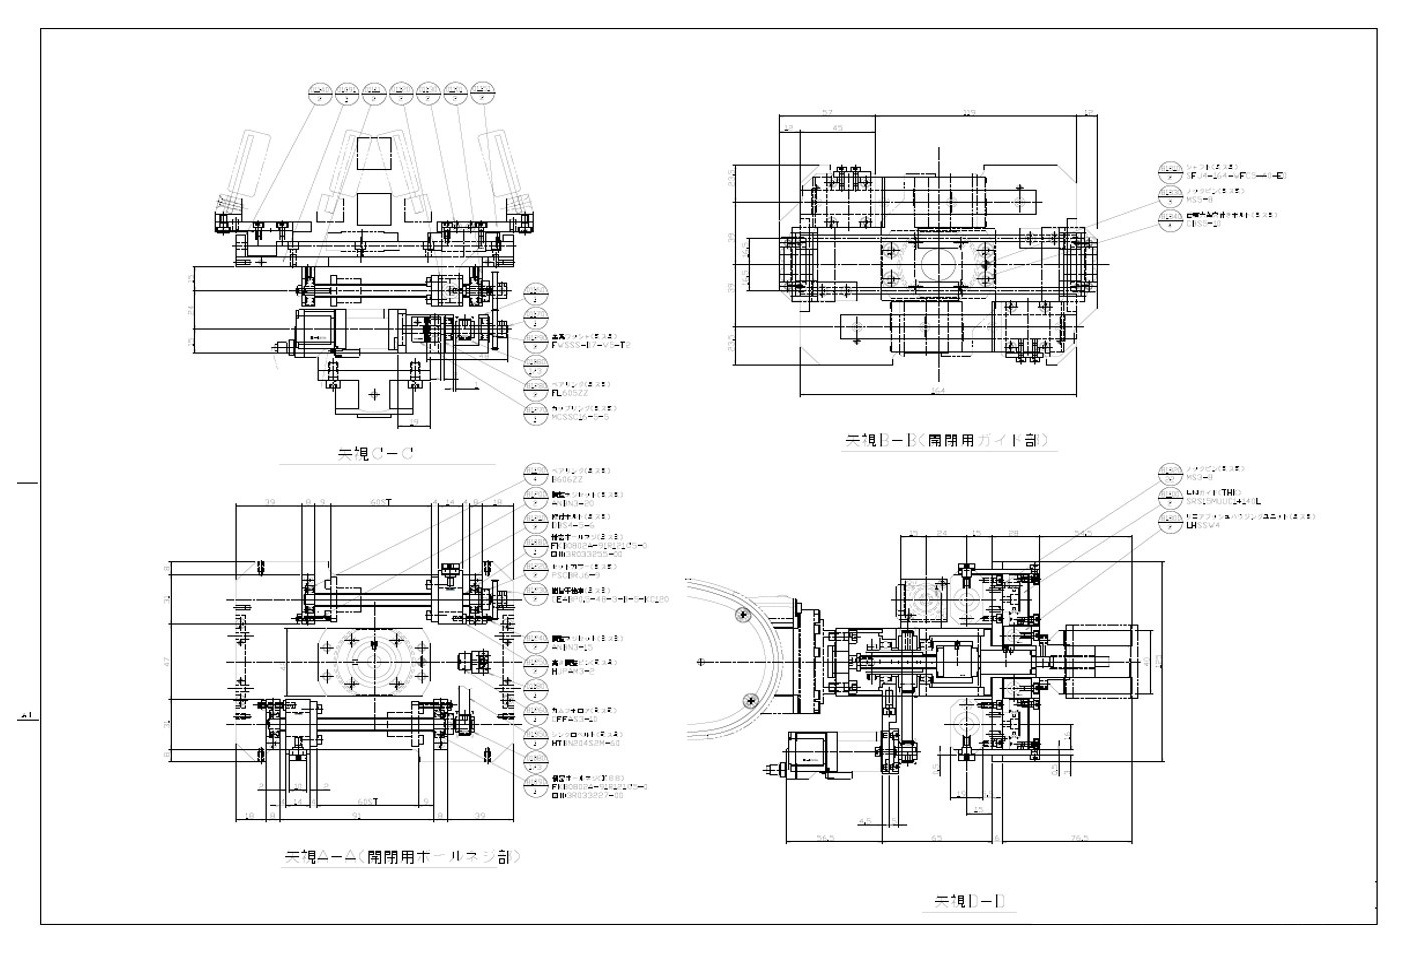
\includegraphics[scale=0.6]{../fig/eps/tercelo_fig.eps}}
\hspace{5mm}
\subfloat[3D図]{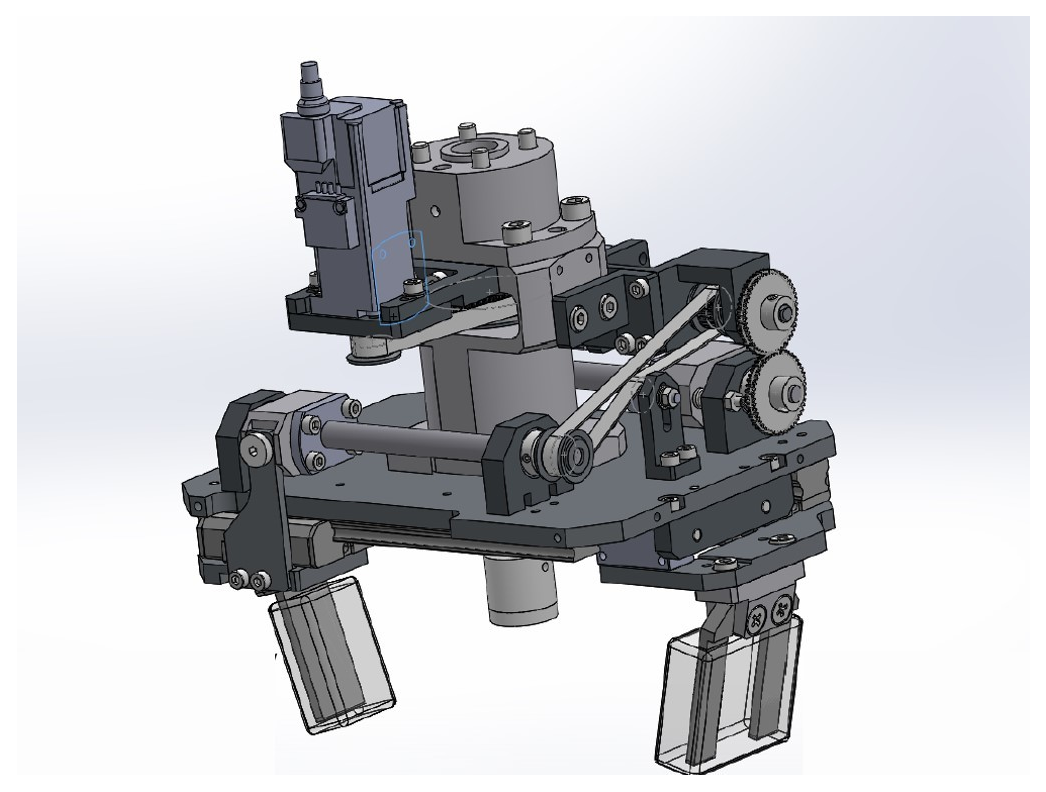
\includegraphics[scale=0.4]{../fig/eps/tercelo.eps}}
\hspace{5mm}
\subfloat[実際のグリッパ]{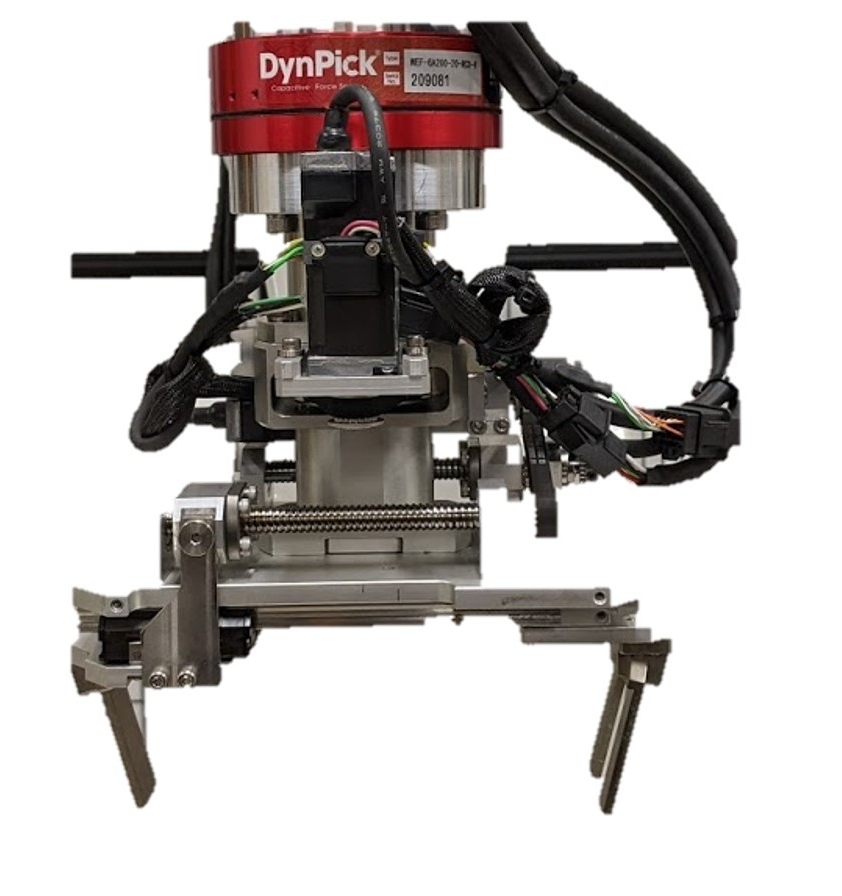
\includegraphics[scale=0.4]{../fig/eps/gripper.eps}}

\caption{内骨格型グリッパ}
\label{fig::gripper}
\end{figure}

\subsection{柔軟指}
本研究では検証に2種類の柔軟指を用いた.いずれも柔軟な把持部にラティス構造を有している.ラティス構造に関しては次の項目で詳しく述べる.3Dプリンタで作成した.使用した3DプリンタはKEYENCE製AGILISTA-3200を用いた.材質はAR-G1H(高硬度シリコン)とした.この材質はショア硬さが35である.主成分はシリコン,アクリルモノマーである.

\subsubsection{通常指}
通常指のCADモデルを\refig{soft_finger_CAD}に実際に作成した指を\refig{soft_finger}に示す.この指は内骨格型グリッパに専用設計された指であるため通常指とした.指上部のスリットに力覚センサを組み込む.

\subsubsection{半球型指}

通常指は対象物に倣うよう設計されているため対象物の荷重が分散しセンシングの感度が疑問視される.ここで高感度で荷重を計測するために半球の凸部とセンサ部が接触するように設計した.この指を半球型指とする.半球型指のCADモデルを\refig{sm_cad},実際に作成した指を\refig{sm}に示す.半球形の把持部の中に通常指と同じパラメータのラティス構造を設けた.

\begin{figure}[h]
\centering
\subfloat[正面]{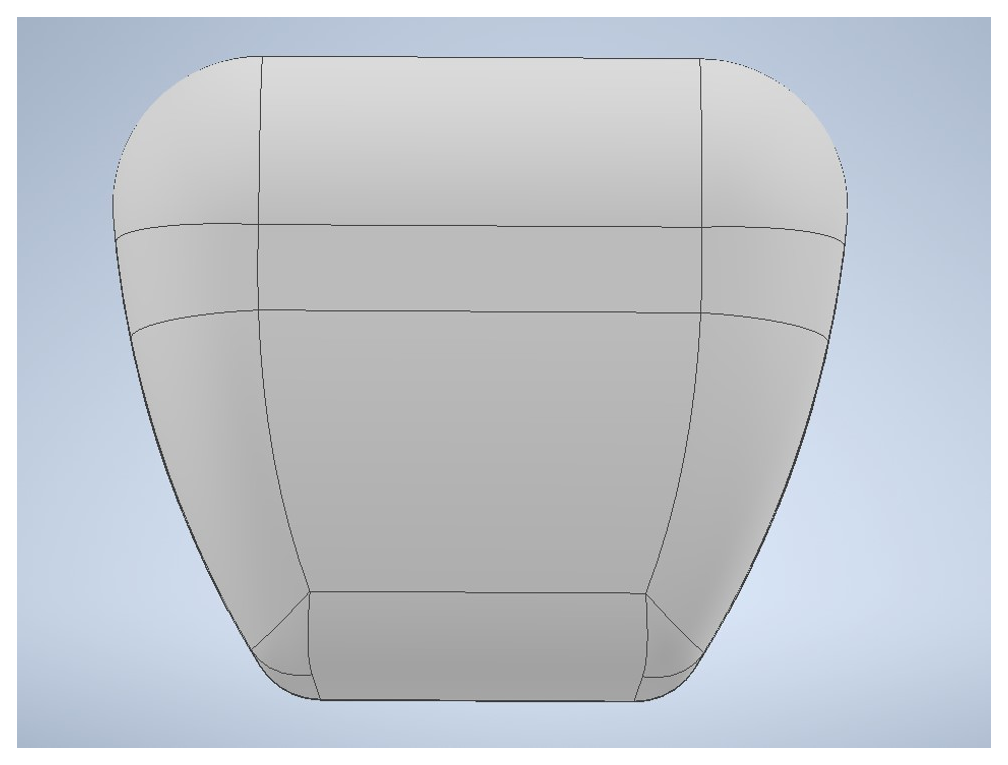
\includegraphics[scale=0.3]{../fig/eps/sf_cad_front.eps}}
\hspace{5mm}
\subfloat[断面図]{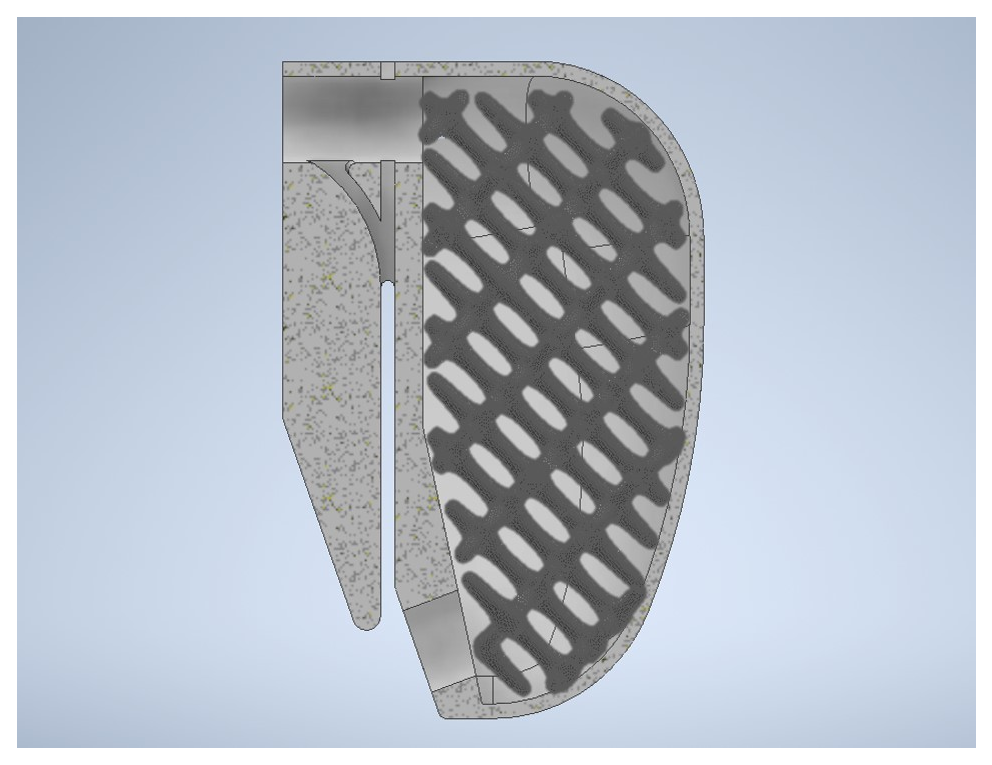
\includegraphics[scale=0.3]{../fig/eps/sf_cad_side.eps}}
\caption{通常柔軟指CADモデル}
\label{fig::soft_finger_CAD}
\end{figure}

\begin{figure}[h]
\centering
\subfloat[正面]{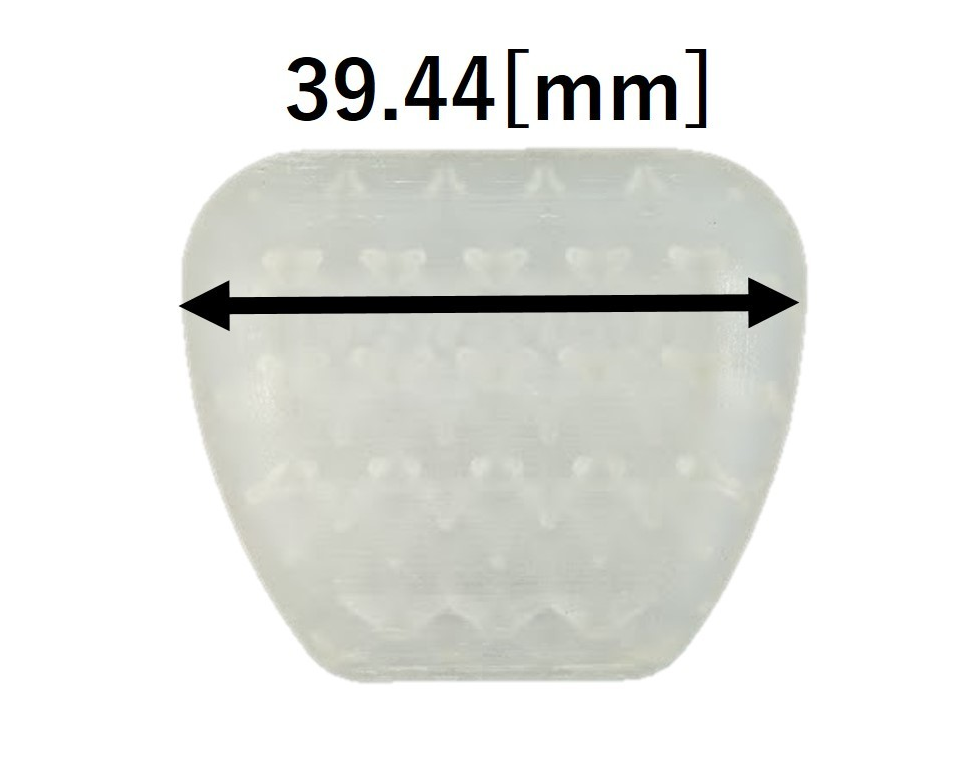
\includegraphics[scale=0.3]{../fig/eps/sf_front.eps}}
\hspace{5mm}
\subfloat[横]{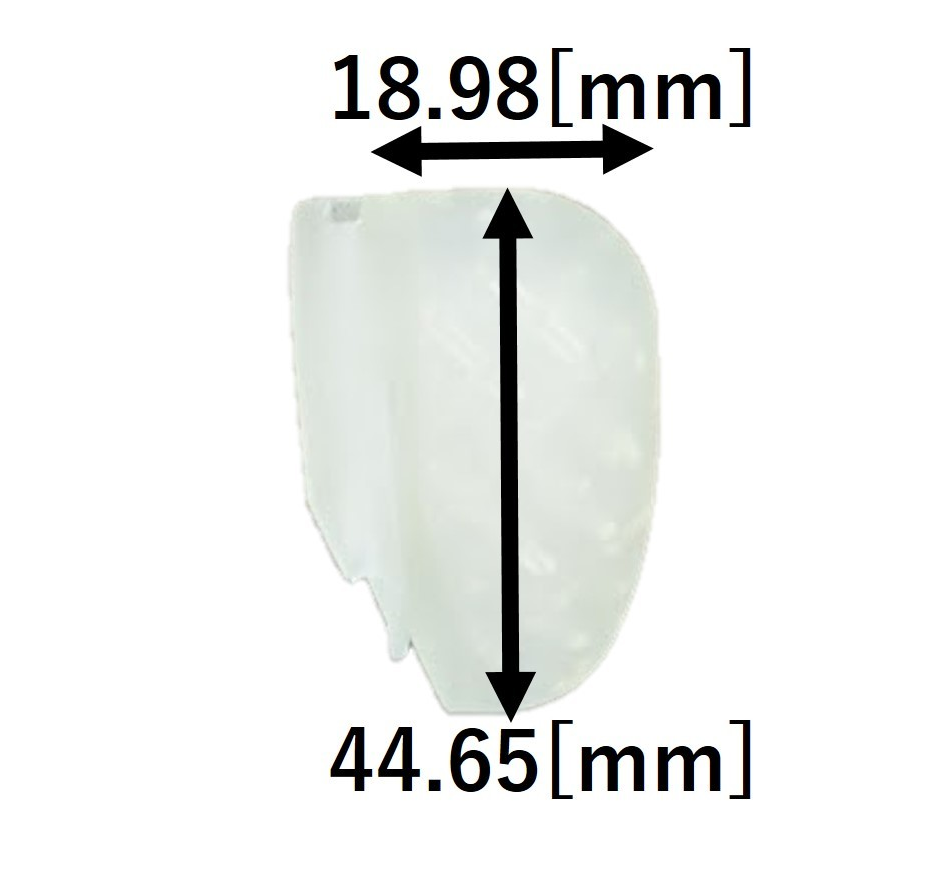
\includegraphics[scale=0.3]{../fig/eps/sf_side.eps}}
\caption{作成した通常柔軟指}
\label{fig::soft_finger}
\end{figure}

\begin{figure}[h]
\centering
\subfloat[正面]{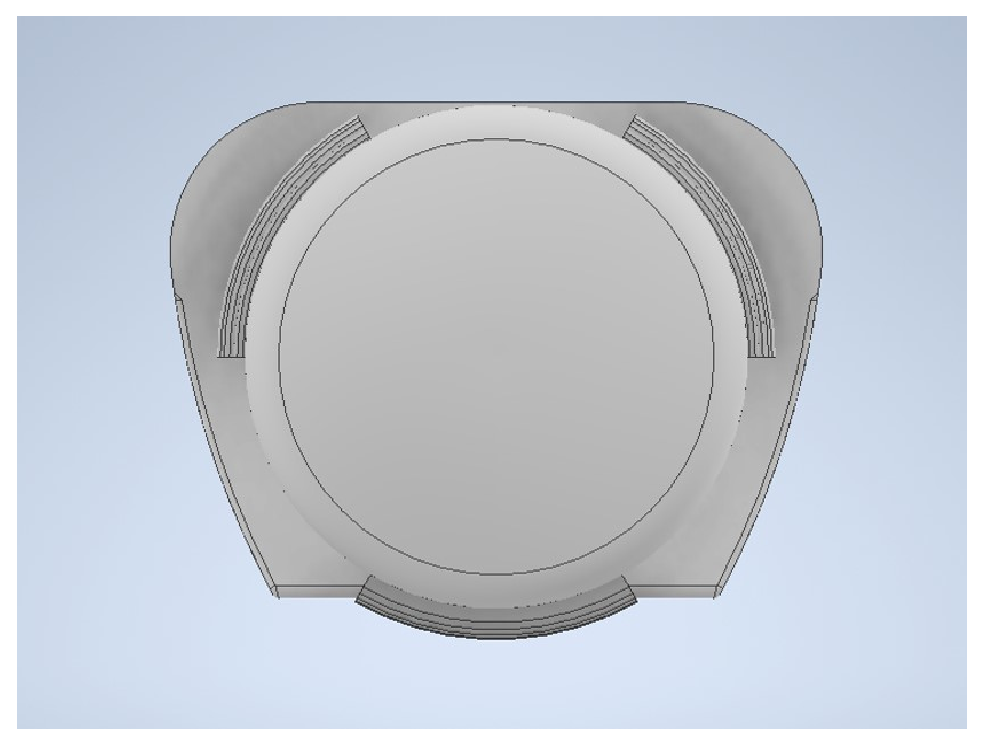
\includegraphics[scale=0.3]{../fig/eps/sm_cad_front.eps}}
\hspace{5mm}
\subfloat[断面図]{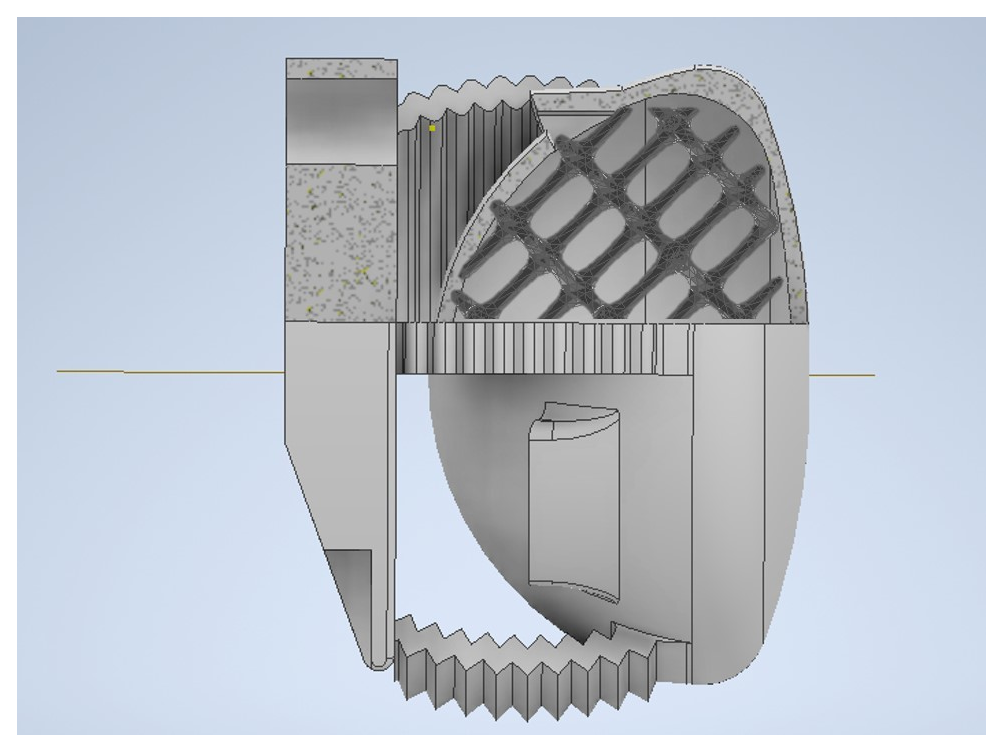
\includegraphics[scale=0.3]{../fig/eps/sm_cad_side.eps}}
\caption{半球型柔軟指CADモデル}
\label{fig:sm_cad}
\end{figure}

\begin{figure}[h]
\centering
\subfloat[正面]{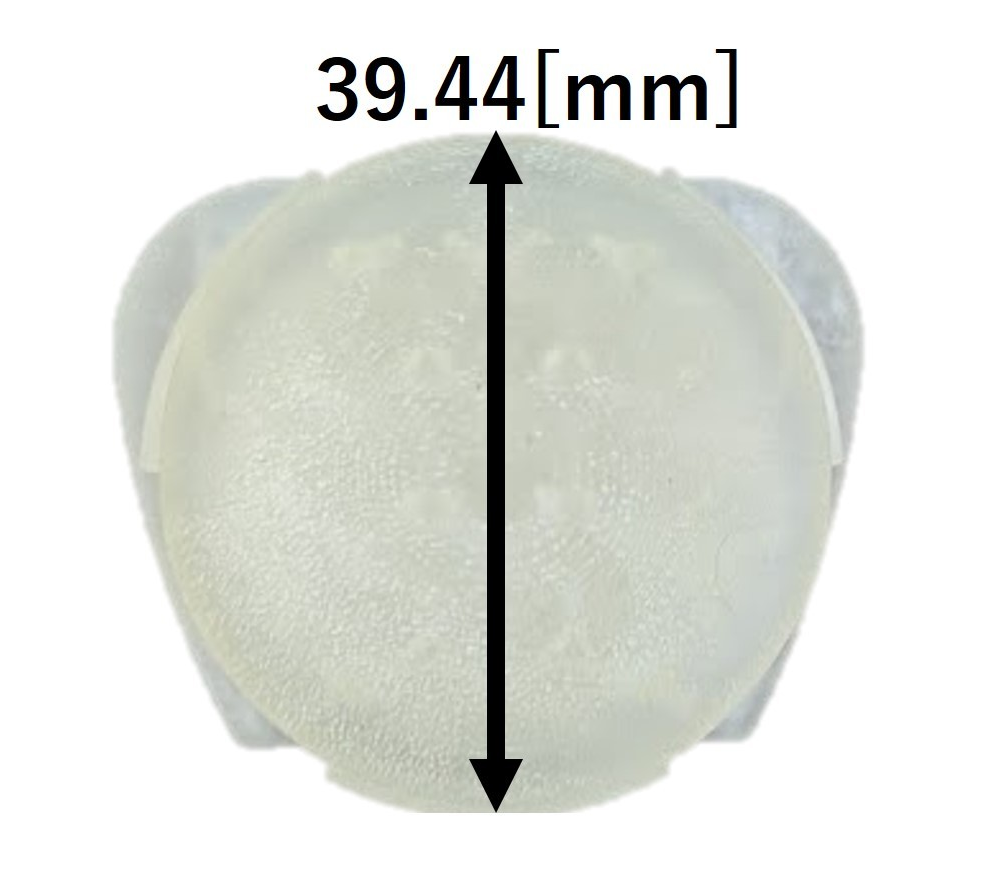
\includegraphics[scale=0.3]{../fig/eps/sm_front.eps}}
\hspace{5mm}
\subfloat[横]{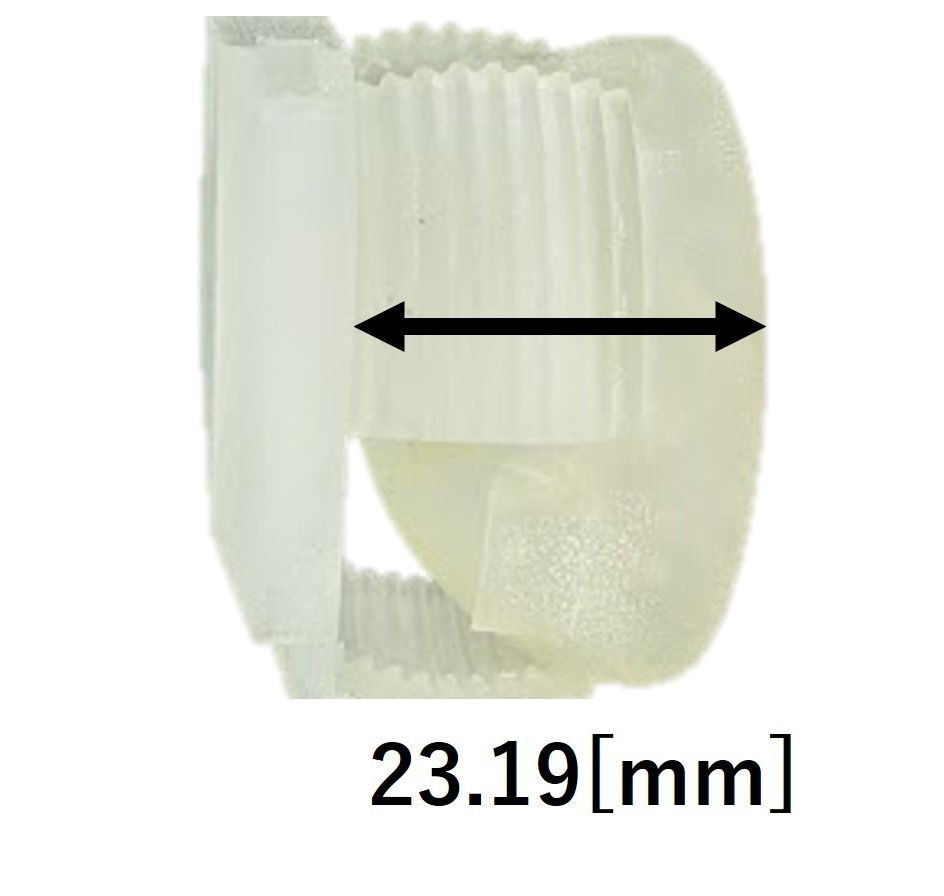
\includegraphics[scale=0.3]{../fig/eps/sm_side.eps}}
\caption{作成した半球型柔軟指}
\label{fig::sm}
\end{figure}

\clearpage

\subsection{ラティス構造}
ラティス構造とは\refig{latice}に示す最小の繰り返し単位が周期的に繰り返される3次元構造で、機械的な強度を損なうことなく軽量化を可能とする\cite{latice}.ラティス構造の特徴として3次元構造の形状や周期のパラメータを変更することができ変形量や内部応答を制御することが可能である.本研究ではAutodesk社製のNetfabbを用いてラティス構造の作成を行いその時のパラメータを\reftab{prm}に示す.


\begin{figure}[h]
\centering
\subfloat[ラティス構造(通常)]{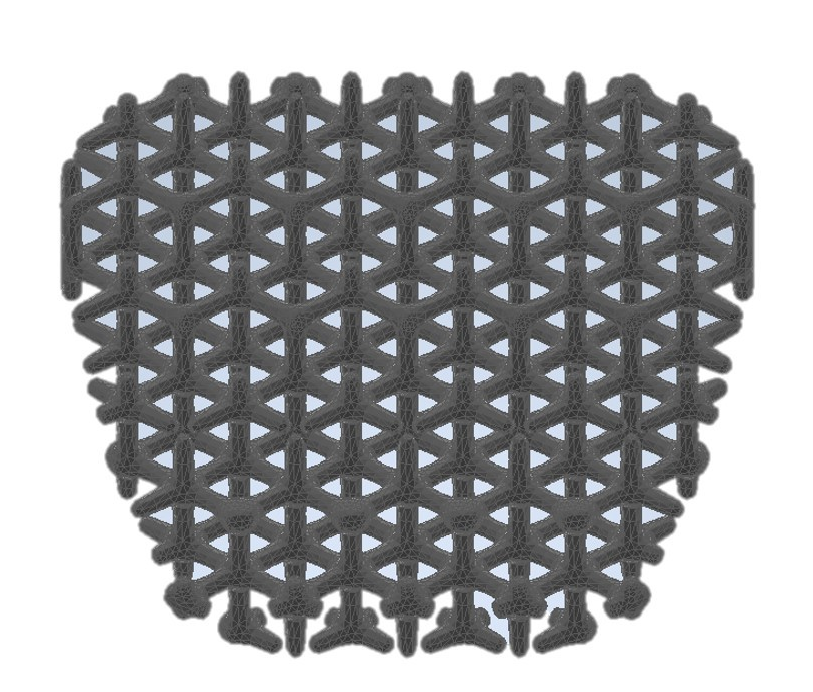
\includegraphics[scale=0.5]{../fig/eps/sf_latice.eps}}
\hspace{5mm}
\subfloat[ラティス構造(半球型)]{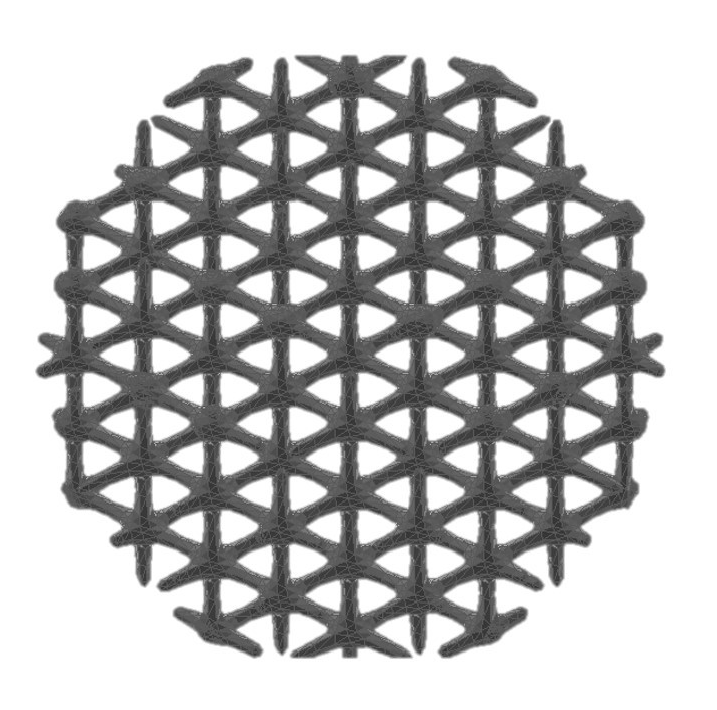
\includegraphics[scale=0.5]{../fig/eps/sm_latice.eps}}
\caption{各指のラティス構造}
\label{fig::latice}
\end{figure}

\begin{table}[htbp]
    \caption{ラティス構造パラメータ} 
  \label{tab::prm}
   %\scalebox{3}[1.5]
  \centering
   \begin{tabular}{|c||c|} \hline
      unit topology & Soft Box  \\ \hline
        Unit size(X,Y,Z) & (8.000mm,8.000mm,8.000mm)  \\ \hline
    Ofset(X,Y,Z) & (0.000mm,0.000mm,0.000mm)  \\ \hline		
    Thickness & (0.671mm)  \\ \hline
    Lattice angle & (0.0deg)  \\ \hline	
    \end{tabular}
\end{table}

\newpage


\subsection{力覚センサ}
イナバゴム社のイナストマーを用いた.\refig{ina}に示す.イナストマーは感圧導電性エラストマー(加圧導電性ゴム)\cite{kanatsu}というゴムを利用した力覚センサである.

\subsubsection{動作原理}
感圧伝導性エラストマーは主にシリコンゴムと導電性粒子(カーボン)から成り立つ.無加圧状態で高い絶縁性を持つが,加圧されるとイナストマーチップ内の導電性粒子が次第に接触しはじめ導電経路が形成され電気抵抗値が低下する.また、減圧して無加圧にするとゴムの弾性による復元力で再度非接触状態に戻る\cite{inabagomu}.

\begin{figure}[h]
\centering
\subfloat[イナストマー]{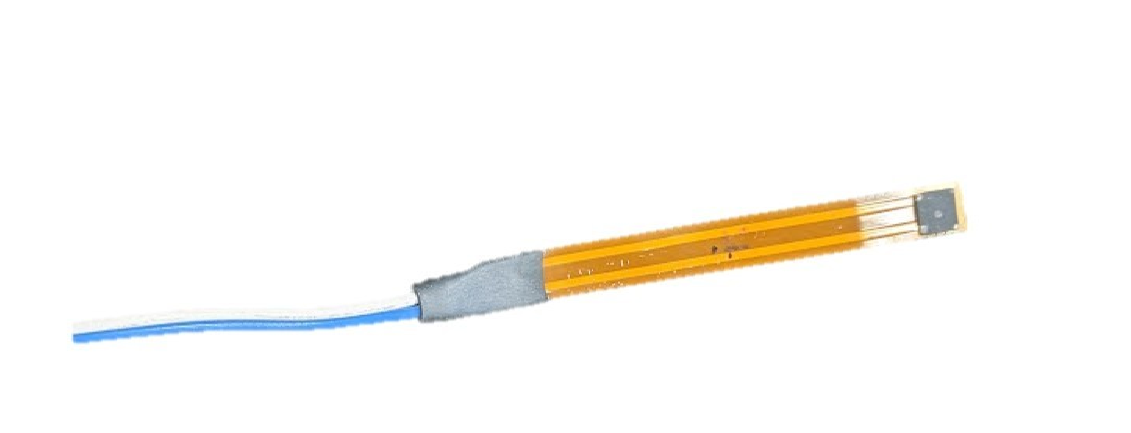
\includegraphics[scale=0.55]{../fig/eps/ina.eps}}
\hspace{5mm}
\subfloat[仕様図]{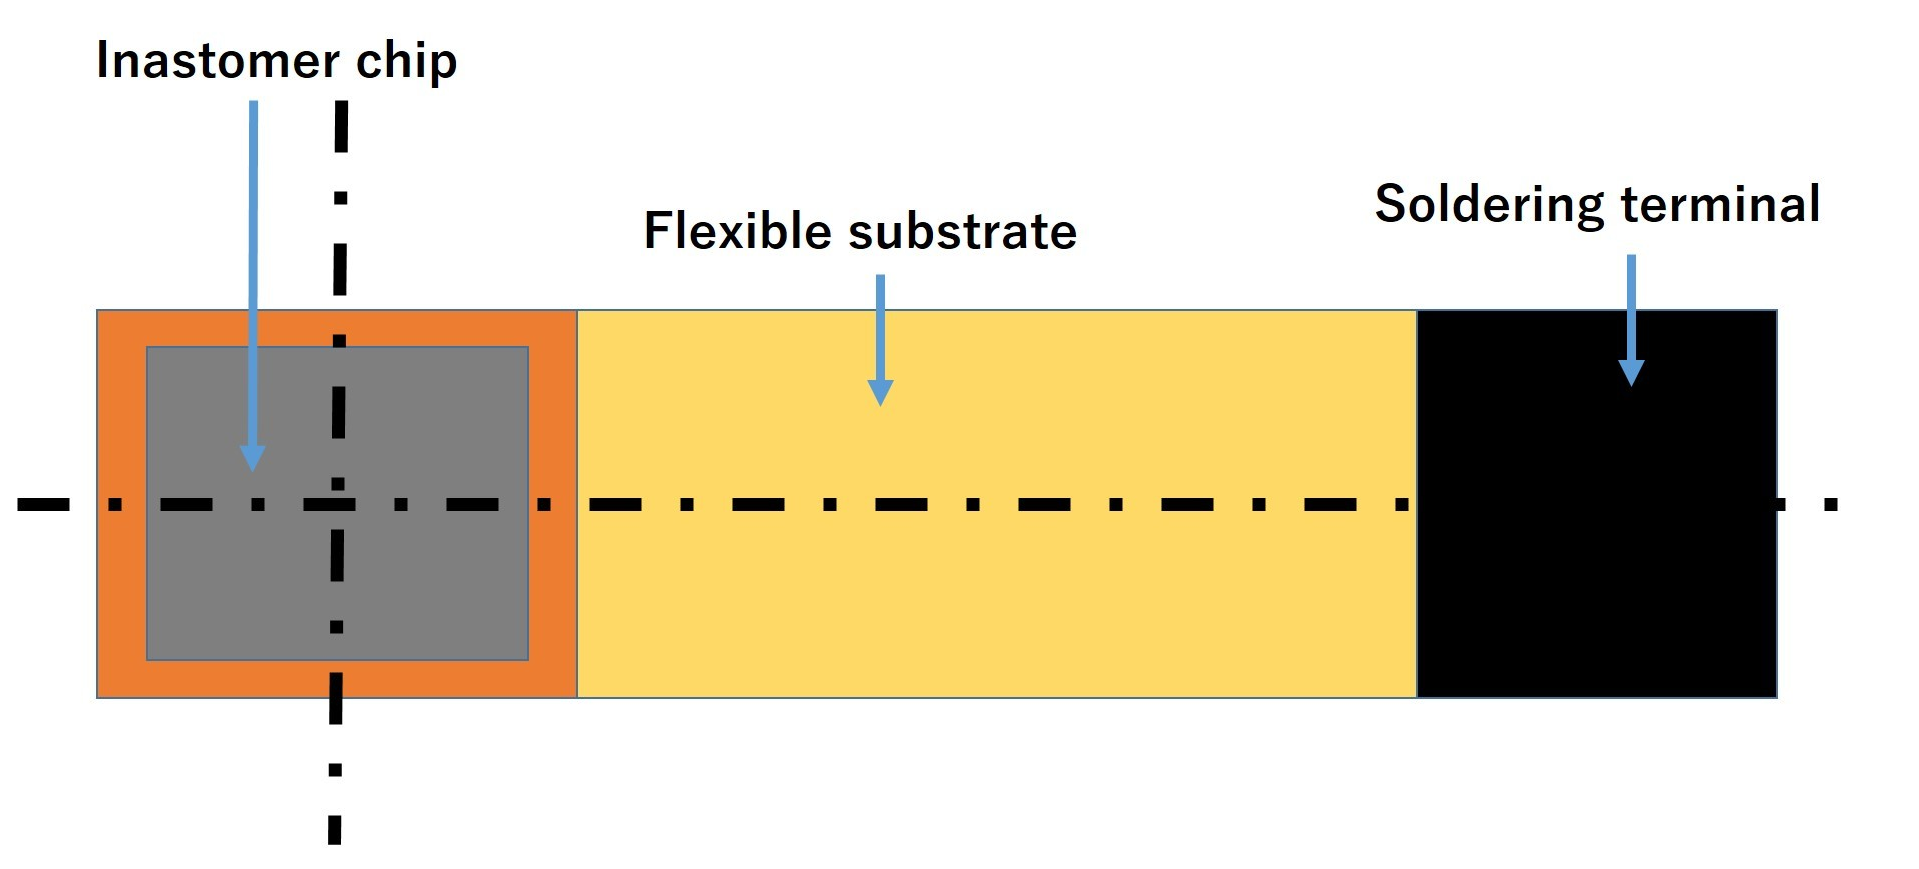
\includegraphics[scale=0.4]{../fig/eps/ina_fig.eps}}
\caption{イナストマー}
\label{fig::ina}
\end{figure}

\newpage



